\section{Исследовательский раздел}

\subsection{Технические характеристики ЭВМ}
Замеры выполнялись на следующей машине:
\begin{itemize}
    \item процессор 11th Gen Intel Core i5-1135G7 4.20 ГГц~\cite{processor};
    \item оперативная память 8 Гб;
    \item операционная система EndeavourOS~\cite{endeavouros} Linux 7.0.3-arch1-2 x86\_64.
\end{itemize}

Указанный процессор имеет 4 физических ядра и 8 логических~\cite{processor}.
Исследование проводилось на ноутбуке, подключённом в сеть, при включённом режиме производительности. При выполнении замеров были запущены лишь системные процессы.

\subsection{Описание исследования}
Проведены два независимых исследования: влияние внешнего кэширования
на время выполнения запросов и влияние индексов на скорость выполнения запросов.

\subsubsection{Исследование влияния кэширования}
Для исследования был выбран запрос получения списка активных ресторанов (листинг~\ref{lst:cache_query}): он выполняется при каждом открытии каталога и при этом обращается к данным, которые меняются редко.

\begin{lstlisting}[language=SQL, caption={Запрос для исследования кэширования}, label={lst:cache_query}]
SELECT * FROM restaurants WHERE is_active = true
\end{lstlisting}

Таблица заполнялась $N$ записями для каждого значения из набора $N \in \{500, 1000, 1500, 2000, 2500, 3000, 3500, 4000, 4500, 5000\}$. Для каждого значения $N$ выполнялось~50 замеров после~5 предварительных запросов. Итоговое время определялось как медиана оставшихся замеров. Время измерялось функцией \code{time.perf\_counter()} стандартной библиотеки Python~\cite{Python,time}. Для PostgreSQL оно включает разбор запроса, построение плана, чтение данных и передачу результата клиенту. Для Redis~--- время операции \code{GET} из оперативной
памяти.

\subsubsection{Исследование влияния индексов}

Для проведения исследования была выбрана таблица \texttt{orders}, поскольку необходимо иметь возможность быстро получать все доставленные заказы конкретного клиента. Так как запрос фильтрует строки одновременно по \code{customer\_id} и \code{status}, для индексации были выбраны оба столбца.

В листинге~\ref{lst:index_query} представлен рассматриваемый запрос, на котором проводились замеры. Значение \code{customer\_id} подставлялось как параметр при каждом вызове. В листинге~\ref{lst:test_index} представлено создание составного индекса в таблице \texttt{orders}.

\begin{lstlisting}[language=SQL, caption={Рассматриваемый запрос}, label={lst:index_query}]
SELECT order_id, total_amount
FROM orders
WHERE customer_id = $1 AND status = 'delivered'
\end{lstlisting}

\begin{lstlisting}[language=SQL, caption={Создание составного индекса}, label={lst:test_index}]
CREATE INDEX idx_orders_customer_status
ON orders(customer_id, status)
\end{lstlisting}

Время выполнения измерялось с использованием команды PostgreSQL \code{EXPLAIN~(ANALYZE,~TIMING)}~\cite{explain}. Перед каждой серией замеров выполнялся \code{VACUUM~ANALYZE}~\cite{vacuum}, чтобы планировщик работал с актуальной статистикой. Объём таблицы варьировался в диапазоне $N \in \{10000, \allowbreak{} 25000, \allowbreak{} 50000, \allowbreak{} 100000,\allowbreak{} 200000, \allowbreak{} 300000, \allowbreak{} 400000, \allowbreak{} 500000\}$ строк. Для каждого $N$ проводилось~30 замеров после~5 предварительных; итоговым значением служила медиана.


\subsection{Результаты исследования}

\subsubsection{Влияние кэширования}

Результаты замеров приведены в таблице~\ref{tab:cache_results}.

\begin{table}[H]
\centering
\small
\caption{Результаты исследования влияния кэширования}
\label{tab:cache_results}
\renewcommand{\arraystretch}{1.3}
\begin{tabularx}{\textwidth}{|r|R|R|}
\hline
\multicolumn{1}{|c|}{\textbf{Кол-во записей}} & 
\multicolumn{1}{c|}{\textbf{PostgreSQL, мс}} & 
\multicolumn{1}{c|}{\textbf{Redis, мс}} \\
\hline
500  & 1.744  & 0.230 \\
\hline
1000 & 3.447  & 0.284 \\
\hline
1500 & 5.252  & 0.397 \\
\hline
2000 & 6.599  & 1.798 \\
\hline
2500 & 8.941  & 2.236 \\
\hline
3000 & 10.761 & 2.757 \\
\hline
3500 & 12.244 & 3.139 \\
\hline
4000 & 14.041 & 3.654 \\
\hline
4500 & 16.294 & 4.072 \\
\hline
5000 & 19.665 & 4.173 \\
\hline
\end{tabularx}
\end{table}

На рисунке~\ref{img:cache_benchmark} представлена диаграмма
сравнения времени выполнения запросов.

\begin{figure}[H]
\centering
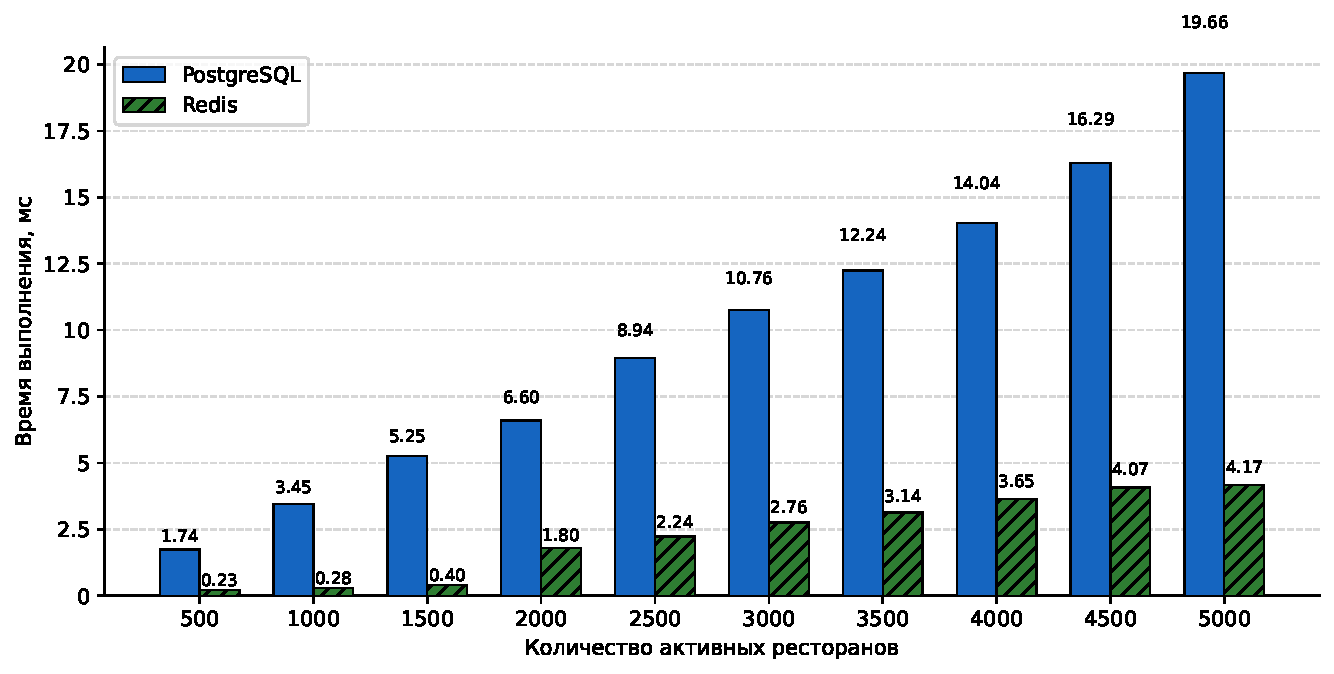
\includegraphics[width=\textwidth]{img/cache_benchmark.pdf}
\caption{Сравнение времени выполнения запроса к PostgreSQL и Redis}
\label{img:cache_benchmark}
\end{figure}

Для измерений PostgreSQL была выполнена линейная аппроксимация методом наименьших квадратов (формула~\ref{eq:cache_approx}):
\begin{equation}
    \label{eq:cache_approx}
    y = 0.0037x + 0.04.
\end{equation}
Коэффициент детерминации $R^2 \approx 0.9998$ подтверждает линейный характер зависимости.
Для Redis коэффициент детерминации составил $R^2 \approx 0.982$, что также говорит о линейном росте времени. Однако время выполнения запросов в Redis растет значительно медленнее --- скорость его роста в 3,75--4 раза меньше (начиная с 2000 записей), чем у PostgreSQL.


\subsubsection{Влияние индексов}

Результаты замеров приведены в таблице~\ref{tab:index_results}.

\begin{table}[H]
\centering
\small
\caption{Результаты исследования влияния составного индекса}
\label{tab:index_results}
\renewcommand{\arraystretch}{1.3}
\begin{tabularx}{\textwidth}{|r|R|R|}
\hline
\multicolumn{1}{|c|}{\textbf{Строк в таблице}} & 
\multicolumn{1}{c|}{\textbf{С индексом, мс}} & 
\multicolumn{1}{c|}{\textbf{Без индекса, мс}} \\
\hline
10\,000  & 0.018 & 0.052 \\
\hline
25\,000  & 0.030 & 0.130 \\
\hline
50\,000  & 0.055 & 0.294 \\
\hline
100\,000 & 0.106 & 0.569 \\
\hline
200\,000 & 0.211 & 1.123 \\
\hline
300\,000 & 0.429 & 1.724 \\
\hline
400\,000 & 0.930 & 2.774 \\
\hline
500\,000 & 1.357 & 3.535 \\
\hline
\end{tabularx}
\end{table}


На рисунке~\ref{img:index_benchmark} представлена диаграмма
сравнения времени выполнения запросов.

\begin{figure}[H]
\centering
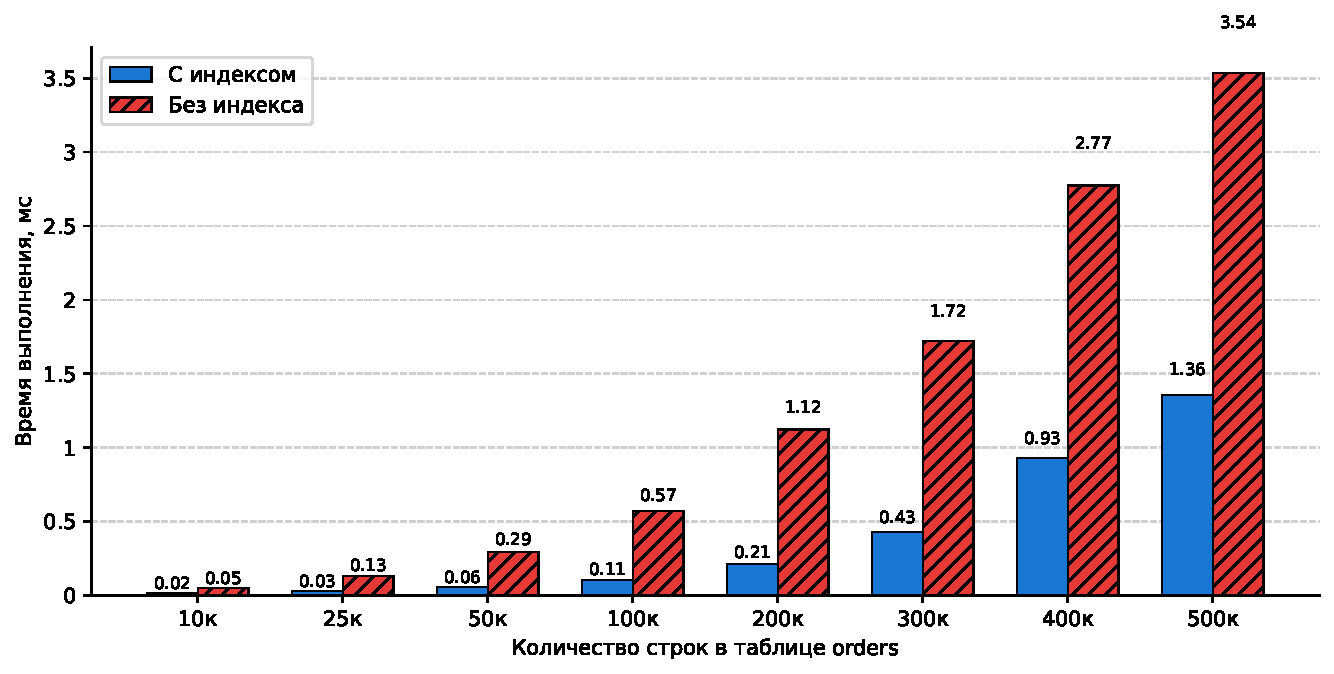
\includegraphics[width=\textwidth]{img/index_benchmark.pdf}
\caption{Сравнение времени выполнения запроса с индексом и без}
\label{img:index_benchmark}
\end{figure}

Запрос с индексом выполняется быстрее на всём исследованном диапазоне.
При 10\,000 строк ускорение составляет 2.9 раза, поскольку оба
варианта работают с данными в памяти. В диапазоне от 25\,000 до
200\,000 строк ускорение стабилизируется на уровне 5.3--5.4 раза:
последовательное сканирование затрагивает всё больший объём страниц,
тогда как индексный поиск обращается только к нужным строкам. При
дальнейшем росте таблицы ускорение снижается до 2.6 раза, так как
при таком объёме оба варианта активно обращаются к дисковым
страницам.


\subsection{Вывод}
В данном разделе приведены технические характеристики устройства, описаны исследования влияния внешнего кэширования и индексов на время выполнения запросов и представлены их результаты. Время выполнения запроса к PostgreSQL растёт линейно с увеличением объёма выборки, тогда как Redis обеспечивает значительно меньший прирост. Составной индекс ускоряет выполнение запросов в 2.6--5.4 раза в зависимости от объёма таблицы.